\chapter*{Appendices}
\addcontentsline{toc}{chapter}{Appendices}

\begin{appendices}
	\appendix
	\renewcommand{\thesection}{\Alph{section}}

	\section{Presenting the hosting organization: \textit{LASS-CNRS}}

	The hosting organization of this internship is the \textbf{Laboratory for Analysis and Architecture of Systems}
	(\textit{Laboratoire d'Analyse et d'Architecture des Systèmes, LAAS}) of the French National Center for Scientific
	Research (\textit{Centre National de la Recherche Scientifique, CNRS}). The LASS-CNRS is a research laboratory
	located in Toulouse, France.

	It was founded in 1968 in a partnership with the University of Toulouse. It's main research areas are in the fields
	of computer science, robotics, automation, micro and nano systems. The laboratory is composed of 829 members divided
	into 6 research departments:

	\begin{itemize}
		\item Decision and Optimization.
		\item Energy management.
		\item Hyperfrequency and Photonics Systems.
		\item Micro, Nano and Bio Technologies.
		\item Networks, Computer Science and Trusted Systems.
		\item Robotics.
	\end{itemize}

	They focus on five main research areas:

	\begin{itemize}
		\item Energy.
		\item Space.
		\item Future Industry.
		\item Health and Environment.
		\item Mobility and Transport.
	\end{itemize}

	\begin{figure}[H]
		\centering
		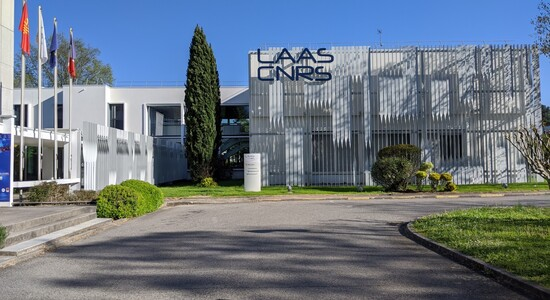
\includegraphics[width=1\textwidth]{../images/LAAS_CNRS_Toulouse.jpeg}
		\caption{LAAS-CNRS front view.\cite{echo-science}}
		\label{fig:laas-front-view}
	\end{figure}

	\begin{figure}[H]
		\centering
		
\includegraphics[width=0.7\textwidth]{../images/logo-laas.jpg}
		\caption{LAAS-CNRS logo.}
		\label{fig:laas-cnrs-logo}
	\end{figure}

\end{appendices}